\section{Models}\label{appendix:models}
The selection of encoder networks includes both standard baselines (ResNet, Vanilla TF) and more specialized architectures (Grid TF, Pondering Looped TF, LLaDA) designed to better capture abstract and spatial reasoning, compositionality, and generalization capabilities.

Table~\ref{tab:encoder_networks_summary} summarizes some of the notable architectural and modeling characteristics used for each encoder network part of the models. The models were designed to roughly have the same size of 1.2 Million of parameters in order to propose a fairer performance comparison, in spite of being aware that different architectures may have different modeling requirements to optimize their performance.

%%%%%% NEW table
\begin{table}[htbp]
  \centering % Center the table horizontally
  % (\ref{tab:encoder_networks_summary})
\begin{tabular}{lccccccc} % {lccccccc} = 1 left-aligned column, 7 centered columns
  \toprule
  % Spanning headers for Architecture and Modeling categories
  & \multicolumn{5}{c}{Architectural} & \multicolumn{2}{c}{Modeling} \\
  \cmidrule(lr){2-6} \cmidrule(lr){7-8} % Rules under the spanning headers only
  Encoder             & APE                 & RPE   & PEMixer      & Recurrence & Diffusion & VT    & Registers           \\
  \midrule
  ResNet        & \textemdash             & \textemdash & \textemdash          & \textemdash & \textemdash & \textemdash  & \textemdash   \\
  Vanilla-TF        & learned             & \textemdash & sum          & \textemdash & \textemdash & \textemdash  & \textemdash   \\
  Grid-TF           & 2D-sincos w/OPE          & RoPE  & vec weighted sum          & \textemdash & \textemdash & \checkmark   & \checkmark    \\
  PL-TF      & 2D-sincos           & RoPE & sum          & \checkmark & \textemdash & \checkmark  & \textemdash   \\
  LLaDA           & \textemdash           & RoPE  & \textemdash          & \textemdash & \checkmark & \checkmark   & \textemdash    \\
  \bottomrule
\end{tabular}
  \caption{Overview of the encoder networks for the different architectural and modeling techniques considered. APE: Absolute Positional Encoding. OPE: Object Positional Encoding. RPE: Relative Positional Encoding. VT: Visual Tokens. Registers: Register tokens. PEMixer: Positional Encoding Mixer, where "vec weighted sum" signifies a vector-weighted sum.}
  \label{tab:encoder_networks_summary}
\end{table}
%%%%%%


%%%%%% OLD table
% \begin{table}[htbp]
%   \centering % Center the table horizontally
%   \caption{Overview of the encoder networks for the different architectural and modeling techniques considered. APE: Absolute Positional Encoding. OPE: Object Positional Encoding. RPE: Relative Positional Encoding. VT: Visual Tokens. Registers: Register tokens. PEMixer: Positional Encoding Mixer, where "vec weighted sum" signifies a vector-weighted sum.}
%   \label{tab:encoder_networks_summary}
%   % (\ref{tab:encoder_networks_summary})
% \begin{tabular}{lccccc} % {lccccc} = 1 left-aligned column, 5 centered columns
%   \toprule
%   % Spanning headers for Architecture and Modeling categories
%   & \multicolumn{3}{c}{Architectural} & \multicolumn{2}{c}{Modeling} \\
%   \cmidrule(lr){2-4} \cmidrule(lr){5-6} % Rules under the spanning headers only
%   Encoder             & APE                 & RPE   & PEMixer      & VT    & Registers           \\
%   \midrule
%   ResNet        & \textemdash             & \textemdash & \textemdash          & \textemdash  & \textemdash   \\
%   Vanilla TF        & learned             & \textemdash & sum          & \textemdash  & \textemdash   \\
%   Grid TF           & 2D-sincos w/OPE          & RoPE  & vec weighted sum          & \checkmark   & \checkmark    \\
%   LLaDA           & \textemdash           & RoPE  & \textemdash          & \checkmark   & \textemdash    \\
%   \bottomrule
% \end{tabular}
% \end{table}
%%%%%%

\subsection{ResNet} \label{sec:resnet_model_details_appendix}
We employ an architecture based on ResNet\citep{he2015deepresiduallearningimage} as a standard baseline notable for its strong historical performances on vision tasks, principally distinguishing itself from the other models evaluated here by its convolutional inductive bias and lack of attention mechanism.

In our implementation, the input grid is processed as a low-resolution image after an artificial channel dimension is created through one-hot encoding of the token categories that can possibly be predicted (i.e., \texttt{num\_token\_categories}). Then, the core of the encoder consists of a sequence of residual blocks. Crucially, all convolutional operations within these blocks are performed without any spatial downsampling (e.g., using stride 1 convolutions and no pooling layers). Despite missing on a slightly more global receptive field, this design choice is important for our tasks, as it strictly preserves the spatial dimensions of the feature maps throughout the network and thus does not require an approach of upsampling. The stacking of convolutional layers without downsampling should also allow the effective receptive field for each individual output pixel to grow, enabling the model to better capture useful context regions while retaining more precise spatial information.

Our specific ResNet architecture comprises:
    \begin{itemize}
        \item An initial convolutional layer to project the input grid channels to the model's hidden dimension: \texttt{num\_token\_categories} input channels, 32 output channels, kernel size of 1, stride of 1, padding of 0. This is followed by Batch Normalization \citep{ioffe2015batchnormalizationacceleratingdeep} and a ReLU activation function \citep{agarap2019deeplearningusingrectified}.
        
        \vspace{1em}
        \item A series of 5 residual blocks:
        \begin{enumerate}
            \item 32 input channels, 64 output channels, kernel size of 3, stride of 1, padding of 1.
            
            \item 64 input channels, 128 output channels, kernel size of 3, stride of 1, padding of 1.

            \item 128 input channels, 128 output channels, kernel size of 1, stride of 1, padding of 0.

            \item 128 input channels, 256 output channels, kernel size of 3, stride of 1, padding of 1.

            \item 256 input channels, 128 output channels, kernel size of 1, stride of 1, padding of 0.
            
        \end{enumerate}

        \vspace{1em}
        \item A final convolutional layer (1x1 convolution) to map the features from the last residual block to the required embed dimension per pixel/token: 128 input channels, \texttt{embed\_dim} output channels, kernel size of 1, stride of 1, padding of 0.

    \end{itemize}
    

\subsection{Vanilla TF} \label{sec:vanilla_vit_model_details_appendix}
We adapt the standard Vision Transformer architecture, as defined in \citep{dosovitskiy2021an}, to our grid-based tasks. The (padded and one-hot encoded) input grid is divided into a sequence of non-overlapping patches, which are effectively single tokens since we use a patch size and stride of 1 when linearly projecting the grid image into the embedding dimension using a 2D convolution.

A basic approach to incorporate spatial information is to use (randomly initialized) 1D learnable positional embeddings to add to the embedded input sequence before it is passed to the encoder network.

This vanilla Transformer encoder consists of multiple layers, each containing a multi-head self-attention (MHSA) mechanism followed by a position-wise feed-forward network. We use Pre-Layer Normalization (Pre-LN) \citep{wang2019learningdeeptransformermodels, xiong2020layernormalizationtransformerarchitecture} and thus apply Layer Normalization before both the MHSA and feed-forward sub-layers. Residual connections are also used around each sub-layer, as is standard. To be able to produce the output grid using an MLP head, a linear layer is applied to each output token of the sequence (from which the special extra tokens have been truncated) at the end of the encoder network in order to map the embedding dimension to that of the MLP head which will then predict the logits for all of the tokens which, once softmax applied and spatially reshaped, form the output grid.

Notable hyperparameters are:
    \begin{itemize}
        \item Input grid partitioning: Patch size of 1, stride of 1. The grid is partitioned at the pixel-level.

        \item Embedding dimension: 128.

        \item Number of encoder layers: 6.

        \item Number of attention heads in MHSA: 4.

        \item Dimensionality of the feed-forward layer: Factor of 4 times the embedding dimension, thus 512.

        \item Activation Functions: GELU \;\citep{hendrycks2023gaussianerrorlinearunits}.

        \item Output projection: A linear layer maps each embed\_dim-dimensional output token (excluding the extra tokens such as the register tokens or the task embedding) to num\_classes logits, where num\_classes depends on the number of tokens to predict (e.g., 15 if Visual Tokens are used, 11 otherwise, as there are ten for the 0-9 symbols and one for padding).
    \end{itemize}


\subsection{Grid TF} \label{sec:grid_vit_model_details_appendix}
The Grid-TF is a variant of the Vision Transformer architecture adapted to improve performance on abstract visual reasoning tasks, especially in grid-like environments, similar to the \generatorName \;data. It incorporates several modifications to improve spatial and abstract visual reasoning. Similar to the Vanilla TF, the input grid is embedded as patches at the pixel level (i.e., patch size and stride of 1 when performing the 2D convolution to transform the grid into an embedded sequence), thus--because deemed inadequate in this context--not exactly appropriating one of the main techniques of Vision Transformers: larger patches.
\newpage
The key architectural modifications from the Vanilla-TF are:
\begin{itemize}
    \item Positional Encodings:
        \begin{itemize}
            \item 2D Absolute Positional Encoding (APE): We use 2D sinusoidal absolute positional encodings, extended from the 1D sinusoidal absolute positional encodings used in \citep{vaswani2017attention}, which are fixed (i.e., not learned) and directly reflect the 2D nature of the input grid. They are added to the patch embeddings following the PEMixer strategy.

            \vspace{1em}
            \item Object Positional Encoding (OPE): OPE is used as part of the APE, as described in \citep{arc_vit} where half of the APE dimension is allocated to the object positions while the other half is used for the x and y positions in the grid. The OPE is also typically coupled with an appropriate PEMixer strategy, such as a vector-weighted sum. We make the choice to compute the object positions \textit{after} having padded (whether with Visual Tokens or with simple padding) the input grid, as opposed to before.

            \vspace{1em}
            \item Positional Encoding Mixer (PEMixer): The PEMixer presented in \citep{arc_vit} defines the strategy by which we encode the absolute positional information into the input embeddings from the absolute positional embeddings. It allows different strategies such as a sum (the standard one), a weighted sum, a vector-weighted sum, etc.

            \vspace{1em}
            \item Relative Positional Encoding (RPE): Due to the importance of the relative positions of the grid tokens when transforming objects, an RPE scheme comes in as a natural consideration. Among possible techniques of RPE, we choose to use Rotary Position Embedding (RoPE) \citep{Su_RoFormer_2024}, incorporated into the self-attention mechanism in order to inject relative spatial information between the grid tokens. After initial experiments with ALiBi \citep{press2022trainshorttestlong}, another RPE method, extended to 2D as in \citep{arc_vit}, we found that RoPE yields comparable performance on our tasks and thus decided to use RoPE for its simplicity.
            
        \end{itemize}
    \vspace{1em}
    \item Registers: We prepend (6) register tokens to the input sequence, following results from \citep{darcet2024vision} and a drawn parallel to slots for object-centric learning in \citep{locatello2020object}. Those registers are additional, randomly initialized and learnable tokens appended to the sequence of patch embeddings in order to possibly improve model performance by functioning as containers for less informative "background" regions of the grid. Thus, they do not correspond to any specific input informing the model and should be leveraged by the attention mechanism to improve global context aggregation and internal representations. The positional encodings are not used for those extra tokens.
                
\end{itemize}

Another modification to the Vanilla-TF is the use of dropout. We apply dropout with a rate of 0.1 after the multi-head self-attention layer and after the feed-forward layer in each Transformer encoder block.

The remaining notable hyperparameters are the same as for the Vanilla-TF.

To better visualize the overall architecture of the Grid-TF encoder, we provide an overview diagram in figure \ref{fig:grid-tf-encoder}.
\begin{figure}
    \centering
    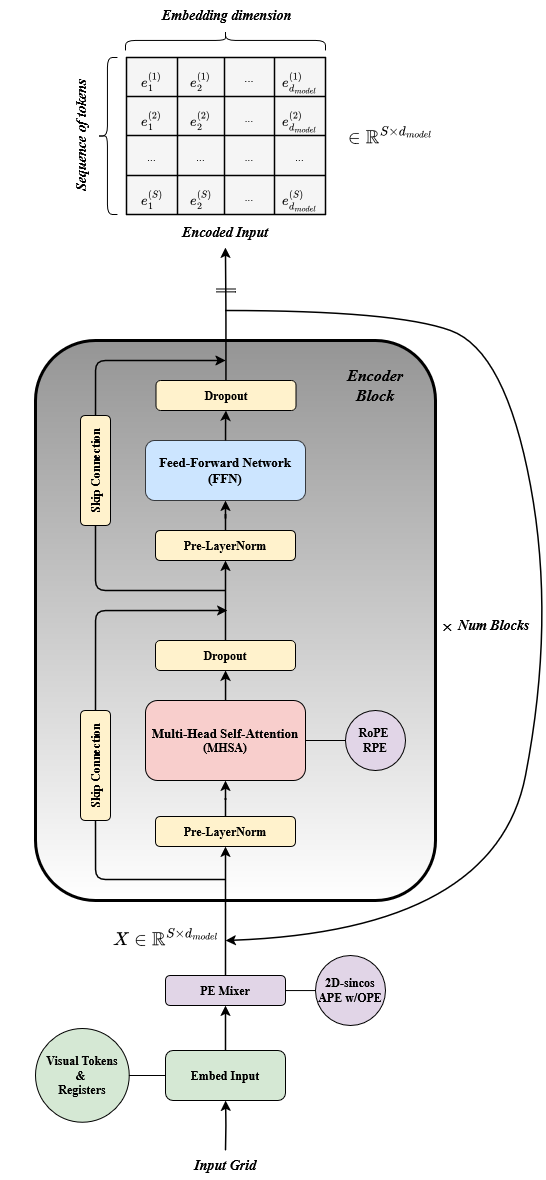
\includegraphics[height=0.9\textheight, keepaspectratio]{Figures/grid_transformer_dropout.png}
    \caption{Overview of the Grid Transformer encoder.}
    \label{fig:grid-tf-encoder}
\end{figure}

\subsection{Pondering Looped TF (PL-TF)}
\label{sec:pl-tf_model_details_appendix}
The Pondering Looped Transformer model closely follows the PonderNet paper by Banino et al. \citep{banino2021pondernet}, using a looped Transformer with weight-sharing as the encoder. As this architecture is less popular than the other ones, we also provide a simplified overview of the architecture in figure \ref{fig:pl-tf-encoder}.

The PL-TF fundamentally differs from the other transformer models in two aspects:
\begin{itemize}
    \item It possesses an inductive bias of recurrent architecture leveraging weight-sharing through an iterative looping process over the same block structure~\cite{dehghani2019universaltransformers, gatmiry2024loopedtransformerslearnimplement, giannou2023loopedtransformersprogrammablecomputers, yang2024loopedtransformersbetterlearning}. At each step, the model updates the latent representation, which can be useful to mimic a multi-stage reasoning process for tasks that require multiple sequential operations on objects.

    \item It makes use of a carefully designed adaptive compute time framework--named PonderNet--controlling the number of iterations and computation effort spent on each data sample~\cite{banino2021pondernet}. Essentially, the model learns a halting probability at each iterative step from an aggregated representation of the current hidden state, which allows it to dynamically and probabilistically decide the number of iterations needed for a given input.
\end{itemize}

\begin{figure}
    \centering
    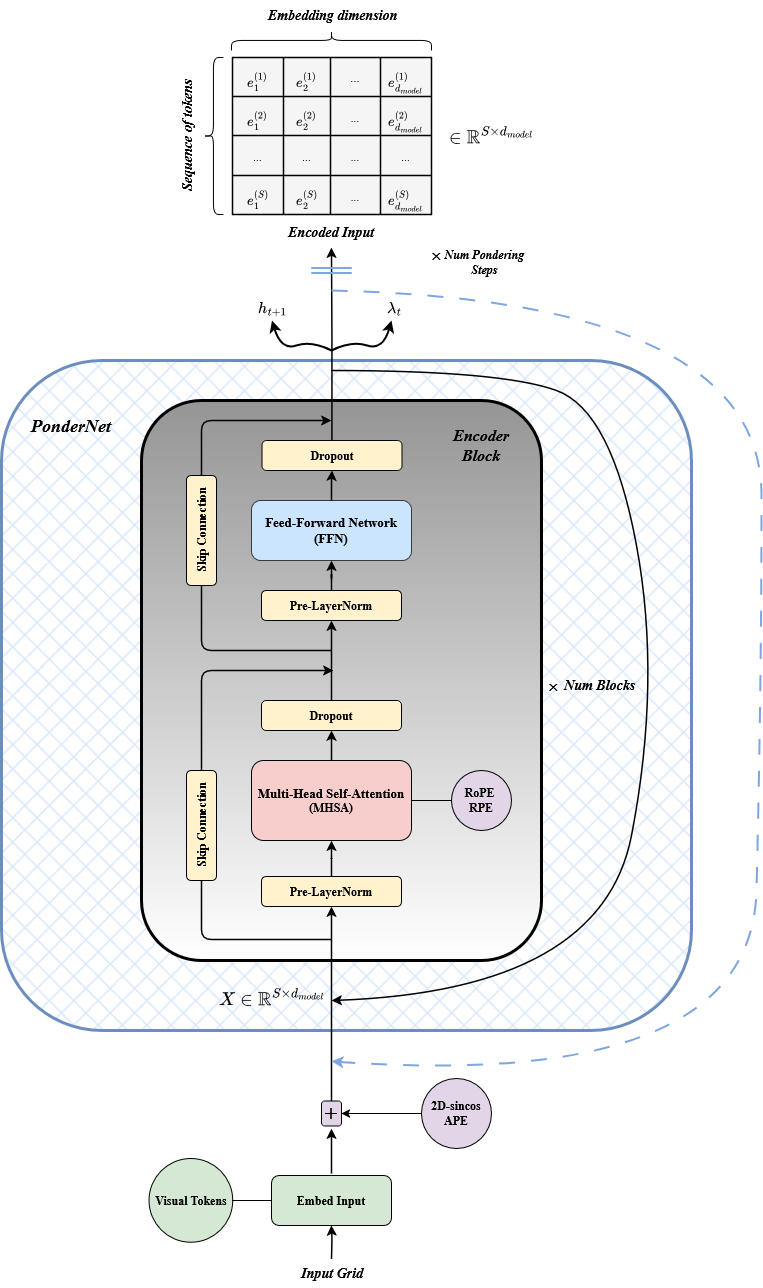
\includegraphics[height=0.9\textheight, keepaspectratio]{Figures/pondering_looped_transformer.png}
    \caption{Overview of the Pondering Looped Transformer encoder.}
    \label{fig:pl-tf-encoder}
\end{figure}

Since parameter-efficiency is not a primary goal, in order to obtain a learnable parameter count comparable to that of the other models, the embedding dimension is set to $d_{model}=256$--instead of $d_{model}=128$ as in the other transformers--and the number of attention heads is set to eight. We use a single encoder block (although more can be used) with weight-sharing.

The computational resource constraints led to the setting of a relatively low maximum number of pondering steps, although a larger maximum number of steps is likely required to fully harness the capabilities of the recurrent and pondering modules. We note that with those decisions the total number of passes through an encoder block is not too far off from that of the other transformers. Furthermore, the pondering-specifc hyperparameters used are: 2-layer halting node with hidden dimension of 128, $\epsilon$ of 0.01, $\lambda_p$ of 0.05, $\beta$ of 0.01.

The encoder block is the same as the Grid-TF with pre-LN, additive skip connections, dropout of 0.1 and a RoPE RPE scheme in the MHSA module. The PL-TF leverages Visual Tokens as the Grid-TF but it uses a 2D sincos APE scheme without object positional encoding or PEMixer.


\subsection{LLaDA} \label{sec:llada_model_details_appendix}
We include LLaDA \citep{Nie_LLaDA_2025} in our set of models due to its demonstrated strength on logical and arithmetic tasks. LLaDA operates non-autoregressively and exploits bidirectional dependencies over masked target sequences, making it well-suited for structured input-output mappings. We adapt the original LLaDA setup skipping pretraining and training it from scratch via supervised learning. Each instance of input data is represented as a flattened concatenation of a task embedding, input sequence, and a partially masked target sequence. During training, a random portion of target tokens is masked (mask ratio sampled uniformly in $[0,1]$), and the model is trained to reconstruct the masked tokens. At inference, the target is fully masked, and reconstruction proceeds over $32$ denoising steps, each resolving a fraction of the masked tokens based on confidence.

In contrast to the original architecture, We use a lightweight $6$-layer version with approximately $1.2$M parameters. The architecture uses an embedding dimension of $128$, a feedforward hidden size of $384$ (MLP ratio of $4$), and $4$ attention heads. The model incorporates RMSNorm \citep{Zhang_Sennrich_2019} with affine parameters and uses SiLU activation functions \citep{Elfwing_SiLU_2018}. Rotary positional embeddings (RoPE) \citep{Su_RoFormer_2024} are applied independently within each transformer layer, using a shared base frequency parameter of $\theta = 500{,}000$. Weights are initialized via the Mitchell method with a standard deviation of $0.02$. No dropout is used throughout training.
The model's vocabulary comprises $12$ tokens, reflecting the tokenized representation used in \generatorName, and includes special tokens for padding and masking.